\documentclass[11pt,english,french]{scrreprt}
\usepackage{lmodern}
\usepackage{babel}
\renewcommand{\familydefault}{\rmdefault}
\usepackage[T1]{fontenc}
\usepackage{ucs}
\usepackage[utf8x]{inputenc}
\usepackage[a4paper]{geometry}
\geometry{verbose,tmargin=3cm,bmargin=3cm,lmargin=2cm,rmargin=2cm,headheight=2cm,footskip=2cm}
\setlength{\parskip}{\smallskipamount}
\setlength{\parindent}{0pt}

\usepackage{amsthm}
\usepackage{booktabs}
\usepackage{amsmath}
\usepackage[unicode=true, pdfusetitle,
 bookmarks=true,bookmarksnumbered=false,bookmarksopen=false,
 breaklinks=false,pdfborder={0 0 1},backref=false,colorlinks=false]
 {hyperref}

\makeatletter
\usepackage{colortbl}
\usepackage{color}
\usepackage[dvipsnames]{xcolor}
\usepackage{wrapfig}
\usepackage{graphicx}
\usepackage{listings}
\usepackage[calcwidth]{titlesec}
\usepackage{fix-cm}
\usepackage{multicol}
\usepackage{verbatim}
\usepackage{moreverb}

\theoremstyle{remark}
  \newtheorem*{rem*}{Remarque}
\theoremstyle{definition}
  \newtheorem*{defi}{Définition}
  \newtheorem{ques*}{Question}[subsection]

\definecolor{MyDarkBlue}{rgb}{0,0.08,0.45}

\lstset{language=C,
	 	basicstyle=\small\ttfamily,
		keywordstyle=\small\ttfamily,
		identifierstyle=,
		commentstyle=\textcolor{OliveGreen},
		columns=fullflexible,
		stringstyle=\small\ttfamily,
		showstringspaces=false,numberstyle=\tiny, breaklines=false, tabsize=4}

\titleformat{\section}[hang]{\sffamily\bfseries}
 {\Large\thesection}{12pt}{\Large}[{\titlerule[0.5pt]}]

\def\thickhrulefill{\leavevmode \leaders \hrule height 1pt\hfill \kern \z@}
\renewcommand{\maketitle}{\begingroup%
    \let\footnotesize\small
    \let\footnoterule\relax
    \parindent \z@
    \reset@font
    \begin{flushleft}
      \huge \sffamily \bfseries\color{orange} \@title
    \end{flushleft}
    \hrule height 1pt
    \begin{flushright}
      \large\sffamily\color{MyDarkBlue}\@author
    \end{flushright}
  \endgroup%
  \setcounter{footnote}{0}%
}

\AtBeginDocument{
  \def\labelitemi{\normalfont\bfseries{--}}
}

\makeatletter
\renewcommand\thesection{\arabic{section}}
\@addtoreset{section}{chapter}
\makeatother

\makeatother
\begin{document}
	
\title{LI310 - TME 1\\
Configuration de connexion TCP/IP sur Linux}
\author{Benjamin BARON}

\setcounter{section}{1}

\maketitle

\section{Les commandes d'administration et de configuration TCP/IP}
\setcounter{subsection}{1}
\subsection{Nom d'hote}
\begin{ques*}
Nom d'hôte de la machine : \lstinline!nostname! $\Rightarrow$ \lstinline!ari-31-313-07.infop6.jussieu.fr!
\end{ques*}
\begin{ques*}
\lstinline!uname -n! $\equiv$ \lstinline!hostname!\\
La commande \lstinline!uname -u! affiche le nom d'hôte de la machine.
\end{ques*}

\begin{ques*}
Le nom d'hôte d'une machine ne peut pas être utilisé tel quel lors de l'envoi d'un paquet.\\
Traduction DNS pour obtenir l'adresse IP correspondante.
\end{ques*}

\subsection{Adresse IP}
Description du fichier \lstinline!/etc/hosts!

Adresse IP \qquad Nom d'hôte \qquad Alias
\begin{itemize}
	\item \lstinline!127.0.0.1! \qquad \lstinline!localhost.localdomain! \qquad \lstinline!localhost!\\
	Adresse réservé à \emph{loopback} (la machine s'envoie des trames à elle-même ; la trame ne sort pas sur le réseau).
	\item \lstinline!::1! Boucle locale lorsque IPv6 est utilisé
	\item \lstinline!132.227.112.xxx! : Adresse IP de la machine définie dans \lstinline!/etc/host!\\
	Alias défini (ici : \lstinline!ari-31-313-07!).
\end{itemize}

\begin{ques*}
Si la machine n'était pas connectée au réseau, elle n'aurait pas l'adresse \lstinline!132.227.112.xxx!.
\end{ques*}

\begin{ques*}
Adresse IP de la machine : \lstinline!132.227.112.135!
\end{ques*}

\begin{ques*}
Adresse IP de classe B ($132 = 128+4 \Rightarrow 10000100$ en binaire)\\
Masque par défaut (masque primaire) associé : \lstinline!255.255.0.0/16!
\end{ques*}

\begin{rem*}
	Les différentes classes d'adresses IP :
\begin{itemize}
	\item Classe A : \lstinline!0!	 \qquad Masque primaire : \lstinline!255.0.0.0!
	\item Classe B : \lstinline!10!	 \qquad Masque primaire : \lstinline!255.255.0.0!
	\item Classe C : \lstinline!110! \qquad Masque primaire : \lstinline!255.255.255.0!
\end{itemize}
\end{rem*}

\begin{ques*}
2.3.4 Réseau non subdivisé. 
\begin{itemize}
	\item Adresse ID du réseau : \lstinline!132.227.0.0/16!
	\item Adresse IP de la première machine : \lstinline!132.227.0.1/16!
	\item Adresse IP de la dernière machine : \lstinline!132.227.255.254/16!
	\item Adresse IP de \emph{broadcast} : \lstinline!132.227.255.255/16!
\end{itemize}
\end{ques*}

\subsection{Configuration de l'interface IP}

\begin{ques*}
Emplacement de la commande \lstinline!ifconfig! : \lstinline!/sbin/ifconfig!
\end{ques*}

\begin{ques*}
Interfaces présentes dans le noyau : \lstinline!cd /sbin ; ./ifconfig -a! \begin{itemize}
	\item \lstinline!eth0! : interface de la carte ethernet
	\item \lstinline!lo! : interface de \emph{loopback}
	\item \lstinline!sit0! : interface utile lors de l'utilisation de IPv6
\end{itemize}
\end{ques*}

\begin{verbatimtab}[4]	
eth0	Link encap:Ethernet		HWaddr 00:19:E0:0D:65:54  
		inet adr:132.227.112.135	Bcast:132.227.112.159	Masque:255.255.255.224
\end{verbatimtab}

\begin{ques*}
Adresse IP de la machine : \lstinline!132.227.112.135!
\end{ques*}

\begin{ques*}
Adresse MAC associée : \lstinline!00:19:E0:0D:65:54!
\end{ques*}

\begin{ques*}
Si machine déplacée sur un autre réseau :\begin{itemize}
	\item Adresse MAC identique (identifiant de carte réseau attribué par le constructeur de la carte réseau
	\item Adresse IP différente (propre au réseau auquel la machine est connectée)
\end{itemize}
\end{ques*}
	
\begin{ques*}
Masques :\begin{itemize}
	\item Masque primaire : \lstinline!255.255.0.0! (adresse de classe B)
	\item Masque du réseau local : \lstinline!255.255.255.224/27!
\end{itemize}

\begin{lstlisting}	
255.255.255.111		00000
netid	subnetid	hostid
\end{lstlisting}

On a alors : 27 bits netid + subnetid
Puisque masque primaire $\neq$ masque de réseau local $\Rightarrow$ subnetting
\end{ques*}

\begin{ques*}
$8+3 = 11$ bits pour identifier le sous-réseau $\Rightarrow 2^{11} \textrm{valeurs} = 2048 \textrm{ sous-réseaux.}$
\end{ques*}

\begin{ques*}
Adresse du sous-réseau sur laquelle la machine est connectée\\
Adresse de la machine ET masque du sous-réseau\\
Ainsi, on a : \lstinline!132.227.112.128/27!
\end{ques*}

\begin{ques*}
Nombre d'hotes : 5 bits \lstinline!hostid! $\Rightarrow 32 - 2$ machines par sous-réseau (ie. chaque salle est un sous-réseau).
\end{ques*}

\begin{ques*}
Il existe un sous-réseau : \begin{itemize}
	\item Adresse IP du sous-réseau : \lstinline!132.227.112.128/27!
	\item Adresse IP de la première machine de ce sous-réseau : \lstinline!132.227.112.129/27!
	\item Adresse IP de la dernière machine de ce sous-réseau : \lstinline!132.227.112.158/27!
	\item Adresse IP de diffusion de ce sous-réseau : \lstinline!132.227.112.159/27!
\end{itemize}
\end{ques*}

\begin{lstlisting}
ifconfig interface [aftype] options | address ...
\end{lstlisting}

\begin{ques*}
L'argument \lstinline!netmask! est optionnel si le masque de l'adresse associé à l'interface peut être déduit de la classe de l'adresse (ie. il n'y a pas eu de découpage).
\end{ques*}

\begin{ques*}
Activation de l'interface \emph{loopback} : \lstinline!ifconfig lo 127.0.0.1!
\end{ques*}

\begin{ques*}
Activation de l'interface \lstinline!eth0! : \\
\lstinline!ifconfig eth0 132.227.112.138 netmask 255.255.255.224!

\lstinline!ifconfig! : permet de configurer les interfaces.
\end{ques*}

\subsection{Routage IP}
\begin{rem*}[concernant la table de routage]
	Destination, passerelle, masque, interface de sortie à utiliser.\\
	Les adresses IP ne changent pas de l'adresse initiale à l'adresse finale quelques soient les passerelles traversées.
\end{rem*} 

\begin{ques*}
	Routage IP direct -- H1 envoie un paquet IP à H2 qui est sur le même sous-réseau
	\begin{figure}[h!]
		\center
		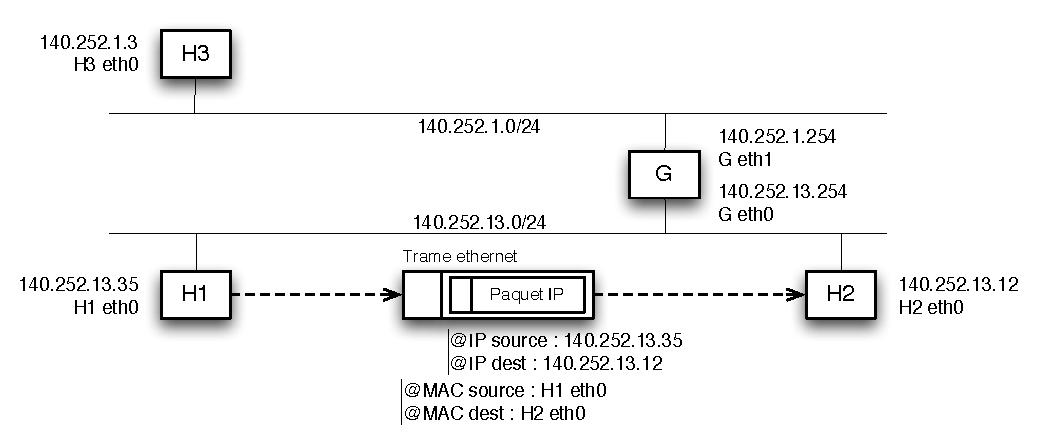
\includegraphics[scale=.8]{graphes/Routage-IP-direct}
	\end{figure}
\end{ques*}

\begin{ques*}
	Routage IP indirect -- H1 envoie un paquet IP à H3 qui est sur un autre sous-réseau
	\begin{figure}[h!]
		\center
		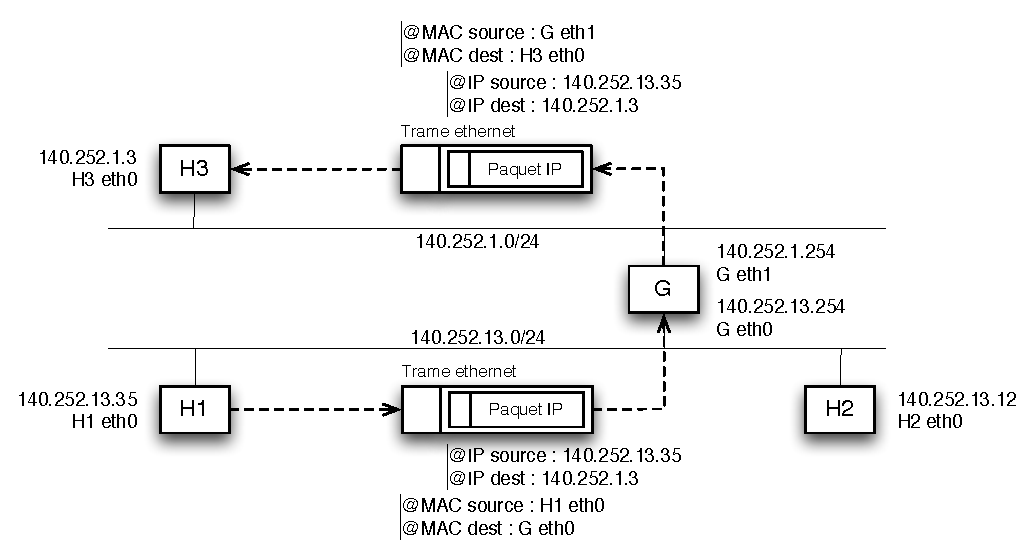
\includegraphics[scale=.8]{graphes/Routage-IP-indirect}
	\end{figure}
	
On peut déduire une adresse MAC à partir d'une adresse IP en utilisant ARP : 
\begin{itemize}
	\item Si Adresse MAC dans le cache ARP $\rightarrow$ OK
	\item Si la correspondance adresse MAC $\leftrightarrow$ adresse IP n'est pas dans le cache :\begin{itemize}
		\item Diffusion sur le réseau local (\emph{broadcast}) d'une requête ARP.
		\item Seule la machine concernée va répondre.
		\item La machine qui a émit la requete va actualiser la correspondance dans son cache ARP.
	\end{itemize}
\end{itemize}
\end{ques*}

\vspace{30pt}

\begin{ques*}
	La commande \lstinline!route! : permet d'afficher la table de routage de la machine
	\lstinline!route -n!

Table de routage IP du noyau
\begin{verbatimtab}[4]
Destination		Passerelle		Genmask			Indic Metric Ref	Use	Iface
132.227.112.128	0.0.0.0 		255.255.255.224 U	  0		 0 		0 	eth0  
/* Adresse du sous-reseau */
169.254.0.0     0.0.0.0			255.255.0.0		U	  0		 0		0	eth0	
/* Adresse reservee : Adressage dynamique lorsque le serveur DHCP est HS */
0.0.0.0			132.227.112.158	0.0.0.0			UG	  0 	 0		0	eth0	
/* Route par defaut */
\end{verbatimtab}
	
	Algorithme de routage :\begin{itemize}
		\item Envoi d'un paquet
		\item Si \lstinline!dest! sur une machine du même réseau $\Rightarrow$ envoi sur le réseau
		\item Sinon envoi sur la route par défaut (ie. le routeur)
	\end{itemize}
\end{ques*}

\begin{ques*}
Adresse de la passerelle du réseau local : \lstinline!132.227.112.158/27!
\end{ques*}


\begin{ques*}
Table de routage : classée par ordre décroissant de la longueur du masque.\\
	Parcours de la table séquentiellement : adresse de destination qui a l'adresse la plus longue (\emph{best matching})
\end{ques*}


\begin{ques*}
	Précision du masque associé au réseau de destination inutile si le masque de l'adresse  destination peut être directement déduit de sa classe.
\end{ques*}

\begin{ques*}
	Argument interface optionnel\\
	Le noyau vérifie si la destination est directement accessible via l'une des interfaces déjà configurées.
\end{ques*}


\begin{ques*}
	Création de l'entrée de la table de routage qui ajoute l'interface \lstinline!eth0!
	\lstinline!route add -net 132.112.128 netmask 255.255.255.224!
	
	\begin{rem*}
		Interface inutile (déjà configurée avant)
	\end{rem*}
\end{ques*}


\begin{ques*}
	\lstinline!route add -net default gw 132.227.112.158!
	\begin{rem*}
		Idem 2.5.8 : interface inutile
	\end{rem*}
\end{ques*}

\begin{ques*}
Les adresses IP contenues dans le fichier 
\end{ques*}


\begin{ques*}
\lstinline!route -C! -- description : \begin{itemize}
	\item Source : entrées pour lesquelles la machine est source
	\item Destination : entrées pour lesquelles la machine est destination (dans les caches de routage, il y a les routes inverses).
	\item Routes inverses : le noyau va anticiper les envois aux machines qui nous ont envoyé des paquets.
\end{itemize}

\end{ques*}

\textbf{Commande \lstinline!netstat!}\\
Outil pour contrôler la configuration d'un réseau et son activité.

\lstinline!netstat -r! : affiche la table de routage (idem \lstinline!route!)\\
\lstinline!netstat -i! : statistiques pour les interfaces réseau configurées\\
\lstinline!netstat -s! : résumé des statistiques pour chaque protocole

\begin{verbatimtab}
Table d'interfaces noyau
Iface       MTU Met    RX-OK RX-ERR RX-DRP RX-OVR    TX-OK TX-ERR TX-DRP TX-OVR Flg
eth0       1500   0    49722      0      0      0    56010      0      0      0 BMRU
lo        16436   0     1576      0      0      0     1576      0      0      0 LRU
\end{verbatimtab}

Taux importants :\begin{itemize}
	\item Taux d'erreur : \lstinline!TX-ERR!
	\item Taux de collision : nombre de collisions / nombre de paquets envoyés (cf. \lstinline!ifconfig!)
\end{itemize}

\begin{rem*}
	Réseau switché $\Rightarrow$ aucune collision.
\end{rem*}

\begin{ques*}
	\lstinline!netstat -nt! : connections TCP actives
\end{ques*}


\begin{verbatimtab}
Connexions Internet actives (sans serveurs)
Proto Recv-Q Send-Q Local Address               Foreign Address             State      
tcp        0      0 132.227.112.135:685         132.227.118.211:48450       TIME_WAIT   
tcp       38      0 132.227.112.135:52249       132.227.87.196:389          CLOSE_WAIT  
tcp       38      0 132.227.112.135:52245       132.227.87.196:389          CLOSE_WAIT  
tcp       38      0 132.227.112.135:52372       132.227.87.196:389          CLOSE_WAIT  
tcp        0      0 132.227.112.135:52374       132.227.87.196:389          ESTABLISHED 
tcp        0      0 132.227.112.135:847         132.227.118.211:2049        TIME_WAIT   
tcp        0      0 132.227.112.135:941         132.227.118.211:2049        ESTABLISHED 
tcp        0      0 132.227.112.135:48406       132.227.87.196:389          ESTABLISHED 
tcp        0      0 132.227.112.135:34909       132.227.118.211:111         TIME_WAIT   
tcp        0      0 132.227.112.135:33476       132.227.118.211:111         TIME_WAIT   
tcp        0      0 132.227.112.135:49812       132.227.118.211:48450       TIME_WAIT   
tcp        0      0 132.227.112.135:44414       132.227.118.211:2049        TIME_WAIT   
tcp        0    152 132.227.112.135:884         132.227.118.214:2049        ESTABLISHED 
tcp        0      0 132.227.112.135:716         132.227.118.214:36396       ESTABLISHED 
tcp        0      0 132.227.112.135:36753       132.227.118.214:111         TIME_WAIT   
tcp        0      0 132.227.112.135:37373       132.227.118.200:3128        ESTABLISHED 
tcp        0      0 132.227.112.135:37374       132.227.118.200:3128        ESTABLISHED 
tcp        0      0 132.227.112.135:37375       132.227.118.200:3128        ESTABLISHED 
tcp        0      0 132.227.112.135:37380       132.227.118.200:3128        ESTABLISHED 
tcp        0      0 132.227.112.135:37379       132.227.118.200:3128        ESTABLISHED 
tcp        0      0 132.227.112.135:37378       132.227.118.200:3128        ESTABLISHED 
tcp        0      0 132.227.112.135:37377       132.227.118.200:3128        ESTABLISHED 
\end{verbatimtab}

A l'ARI : utilisation de proxy $\rightarrow$ utilisation du port 3128 au lieu du port 80 pour \lstinline!http!

\subsection{Cache ARP}
Maintenir un cache ARP
Requête ARP : cher en ressource (bande passante) ; requête ARP traitée par toutes les machines du sous-réseau (consommation du traitement sur les machines du réseau local).

Correspondance IP $\Leftrightarrow$ MAC pour le routeur
\begin{verbatimtab}
Address                  HWtype  HWaddress           Flags Mask            Iface
ari-31-313-06.infop6.ju  ether   00:19:E0:0E:73:11   C                     eth0
ari-31-313-gw.infop6.ju  ether   00:16:47:5A:4D:CA   C                     eth0
\end{verbatimtab}

Créer manuellement une entrée permanente
\lstinline!arp -H ether -i eth0 -s [getwayname or IP] hw_addr!

\section{DNS}

Annuaire réparti et hiérarchique :\\
Nom d'une machine $\rightarrow$ adresse IP

DNS inverse : Adresse IP $\rightarrow$ nom d'une machine

Appel aux DNS : effectués par les processus clients (eg. navigateur internet effectue une requête DNS -- processus transparent pour l'utilisateur).

Commande \lstinline!host www.google.fr!

\begin{verbatimtab}
www.google.fr is an alias for www.google.com.
www.google.com is an alias for www.l.google.com.
www.l.google.com has address 74.125.230.84
www.l.google.com has address 74.125.230.80
www.l.google.com has address 74.125.230.82
www.l.google.com has address 74.125.230.83
www.l.google.com has address 74.125.230.81
www.l.google.com has IPv6 address 2a00:1450:8002::69
\end{verbatimtab}

Le serveur web de google est miroré (il existe des sites miroirs : le site www.google.fr est dupliqué).

Commande \lstinline!dig www.google.fr! : plus d'informations que la commande \lstinline!host!
Quatre sections :\begin{itemize}
	\item Autorité : Serveurs DNS qui gèrent le domaine cherché.
	\item Informations additionnelles : Adresse IP d'un serveur DNS ayant autorité sur le domaine google.com
\end{itemize}

\begin{verbatimtab}
Serveurs de nom primaire
google.com.             67404   IN      NS      ns2.google.com.
google.com.             67404   IN      NS      ns1.google.com.
google.com.             67404   IN      NS      ns3.google.com.
google.com.             67404   IN      NS      ns4.google.com.
\end{verbatimtab}

Adresse IP du serveur primaire : on ne peut pas car la commande dig ne fait pas de distinction entre les serveurs primaires et les serveurs secondaires.

Grace à la commande dig, on peut trouver les serveurs de mail d'un domaine :
\lstinline!dig free.fr mx!

\begin{verbatimtab}
free.fr.                86351   IN      MX      20 mx2.free.fr.
free.fr.                86351   IN      MX      10 mx1.free.fr.
\end{verbatimtab}

Commande \lstinline!host 212.27.48.10! : operation inverse de \lstinline!host www.free.fr!

\lstinline!10.48.27.212.in-addr.arpa domain name pointer www.free.fr!

Il existe 13 serveurs racine : \lstinline!http://www.root-servers.org/!

\section{Commandes de déboguage} % (fold)

 
Commandes \lstinline!ping! et \lstinline!traceroute!

\begin{itemize}
	\item \lstinline!unknown host! : hôte inconnu $\Rightarrow$ Serveur local/distant (ayant autorité) fautif; problème réseau entre serveur local et serveur distant
	\item \lstinline!network unreachable! : réseau inatténiable : problème de routage (vérifier les tables de routage)
	\item \lstinline!no answer! : 100\% de perte $\Rightarrow$ machine cible n'est pas active.
\end{itemize}

\lstinline!ping -b! : ping en broadcast (ie. envoyer un ping à toutes les machines connectées au même réseau).

$\Rightarrow$ envoi d'un paquet \lstinline!ECHO_REQUEST!

Autant de \lstinline!ECHO_REPLY! que de machines sur le réseau => la machine émettrice de l'\lstinline!ECHO_REQUEST! va crouler sous les réponses \lstinline!ECHO_REPLY!

\end{document}
